\documentclass{article}
\usepackage{ctex}
\usepackage{graphicx}
\usepackage{amsmath}
\usepackage{indentfirst}
\usepackage{titlesec}
\usepackage{setspace}
\usepackage{subfigure}
\usepackage{caption}
\usepackage{float}
\usepackage{booktabs}
\title{\songti \zihao{2}\bfseries 全息显微技术近况的调研}
\titleformat*{\section}{\songti\zihao{4}\bfseries}
\titleformat*{\subsection}{\songti\zihao{5}\bfseries}

\author{王启骅 PB20020580}
\linespread{1.5}
\begin{document}
	\maketitle
	\begin{abstract}
		\kaishu\zihao{-5}\quad 全息技术适用于各种形式的波动,尤其是光学全息术自从诞生以来在各个领域有着多样的应用,如立体电影、显微术、军事侦察监视、金属内部探测等。本文调研了当今全息显微技术的前沿状况,主要讨论了数字全息显微镜在微生物探测、与深度学习结合方面的应用。
		
		
	\end{abstract}
	\hspace{1.4cm}\heiti\zihao{-5}\quad 关键词:
	\kaishu\zihao{-5}全息光学;全息技术;数字全息显微镜;深度学习
	\section{引言}
	\songti\zihao{5}
全息显微术是全息与显微相结合的技术。与一般显微术相比,尤其是对一些活的标本物,它可以用高功率的连续光或脉冲激光拍照全息图,长期保存, 再现像具有立体性, 能显示样品的细节。全息显微术广泛应用于医学、生物学、科研等方面。

	
	
	全息显微术主要有的2种形式: 一种是将全息技术和显微镜结合, 称为“全息显微镜”, 解决了一般显微镜中分辨本领与景深的矛盾, 避免了像差影响而达到很小衍射极限, 可以获得更大的视野; 一种是利用全息图本身的特性来进行放大, 称为“全息放大”。本文将着重讨论第一种形式。
	\section{数字全息显微镜}
	

	\songti\zihao{5}\indent
全息显微镜通过让样品束和参考光束进行干涉以产生干涉图案或全息图来创建(定量)相位图像,如下图所示。	使用高分辨率图像传感器以数字方式记录全息图,再使用计算机创建全息影像,以产生最终相位图像。
  \begin{figure}[!h]
	\centering
	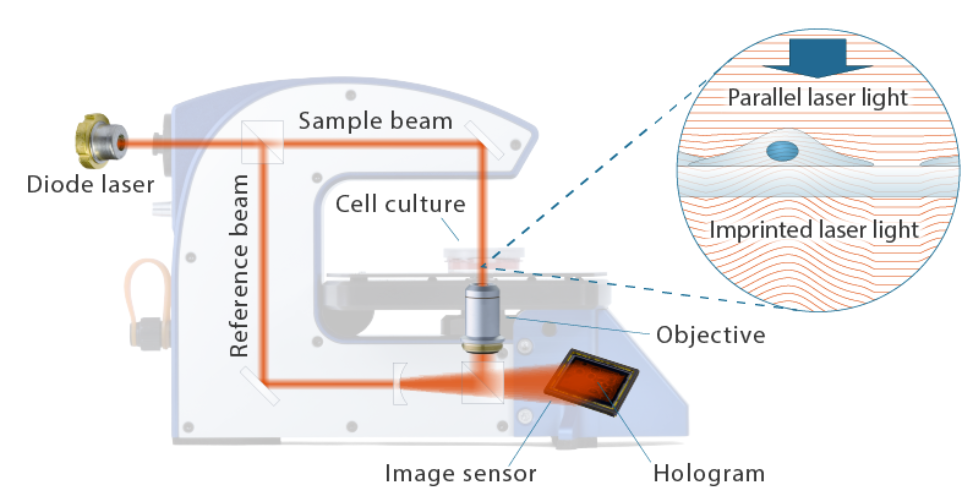
\includegraphics[scale=0.4]{全息显微镜原理图}
	\captionsetup{font={small},labelfont=bf}
	\caption{\heiti\zihao{-5}全息显微镜原理图}
	
\end{figure}
\subsection{数字全息在微生物观察方面应用}
\songti\zihao{5}\indent 在地外生命的探测需要对如细菌等原核生物的识别,而传统光学显微镜受限制于易受环境条件影响、体积质量大、需要精细操作等难以在地外环境使用。而数字全息显微镜有大景深,数值聚焦,能进行定量振幅与相位成像等诸多优势,成为地外生命探测的首选。其中主要存在以下几种类型。

\begin{figure}[!h]
	\centering
	\subfigure[共模“离轴”数字全息显微镜]{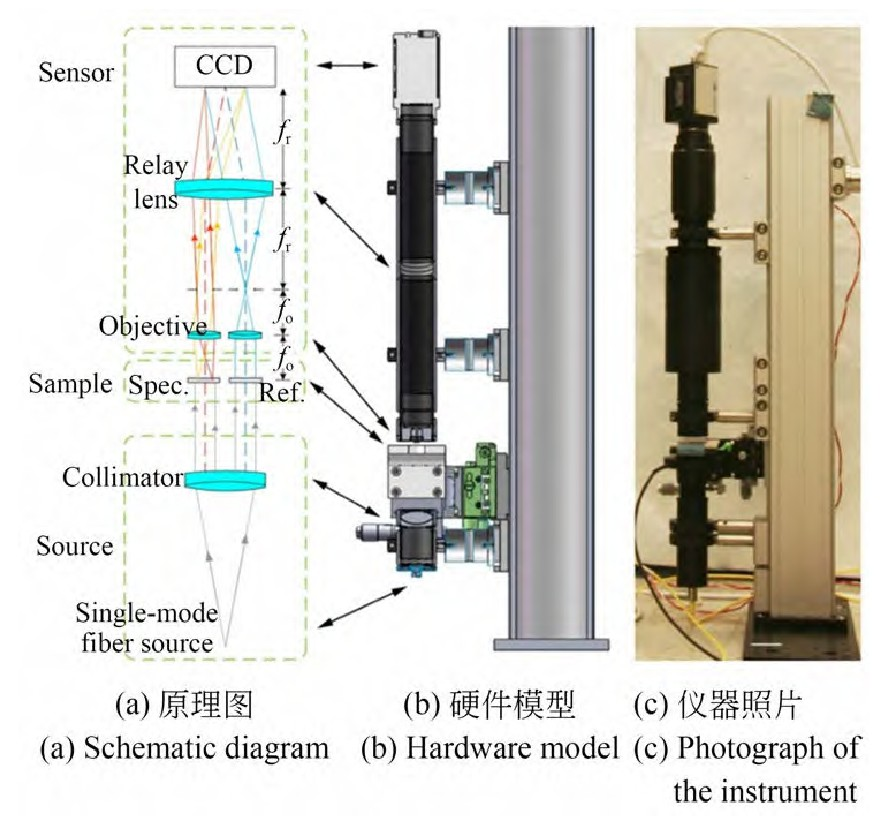
\includegraphics[scale=0.6]{共模}}
\subfigure[无透镜数字全息显微镜]{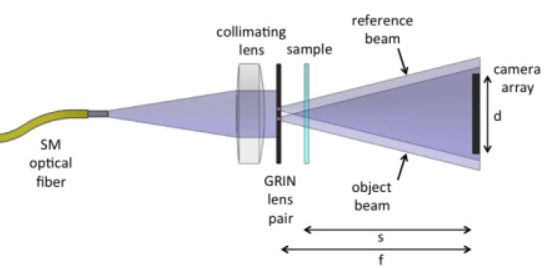
\includegraphics[scale=0.6]{无透镜}}
	\subfigure[并行相移数字全息显微镜]{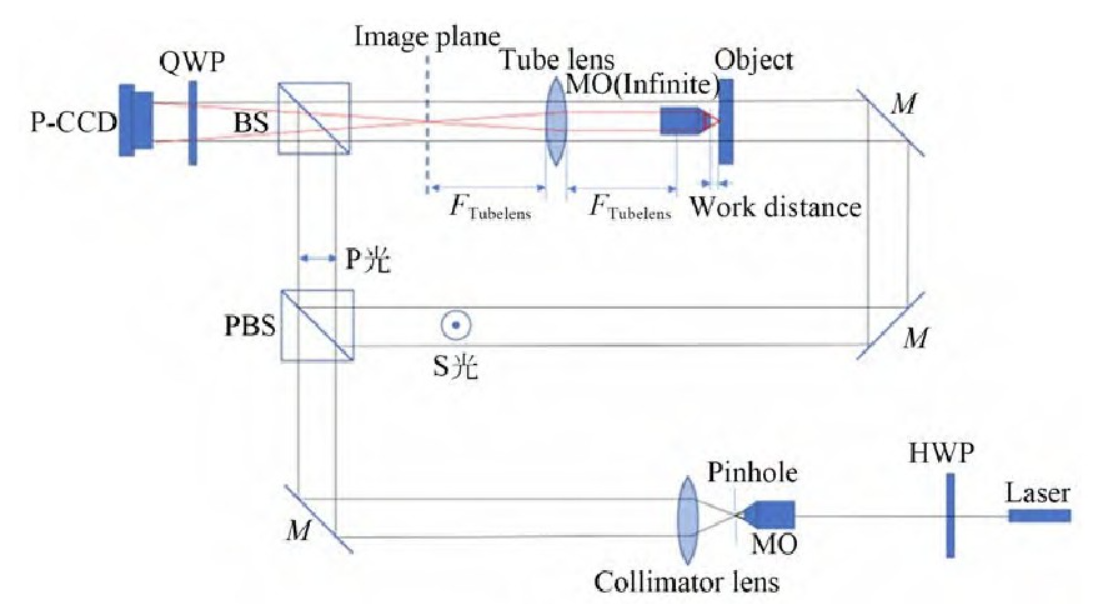
\includegraphics[scale=0.25]{并行}}
	
	\captionsetup{font={small},labelfont=bf}
	\caption{\heiti\zihao{-5}数字全息显微镜}
	
\end{figure}
共模“离轴”数字全息显微镜主要由纤维单色光源、准直透镜、物镜和管透镜组成。纤维光源发出的光束先经过准直透镜变为两束平行光,分别经过观察样品和参照物,之后经过物镜放大,最后管透镜将平行物光和参考光束以一定的夹角汇聚到CCD处进行离轴干涉。但数字全息显微镜仅可以判断原核生物的物理性质结构,无法获得其化学组成。2019年Gene Serabyn团队将其与荧光场显微镜结合的双模式生命探迹体成像系统,先通过数字全息臂观察细菌生命活动,再对细菌染色后通过荧光臂观察得到核酸与细胞膜脂类组成。


无透镜数字全息显微镜主要特点为参考光束和源光束直接照亮探测器阵列,无需任何干预光学器件。图2(b)为2016年Serabyn团队搭建的紧凑型无透镜数字全息显微镜,也采用离轴光路。光源经过准直透镜后,准直光束照亮一对自聚焦透镜(Grin Lens),在焦平面产生一对高NA焦点。用单个准直光束照亮两个GRIN透镜,消除了对第二根光纤的需求,并使系统在光纤尖端之前一直处于共模状态,从而消除了双光纤系统容易受到的潜在路径长度漂移的影响。从共面输出焦点,两束光束以高数值孔径扩展以穿过样品后到达相机。由于光源对和检测器阵列之间没有光学元件(样品除外),成像载物台本身确实是无透镜的。


并行相移数字全息显微镜。2020年中科院长春光机所孟浩然团队提出了基于光波偏振属性的并行相移数字全息技术。该技术在原有系统上增加无限共轭显微模块,利用其中管透镜对物镜引入的二次位相畸变进行物理补偿,可降低数字全息显微镜算法的实现难度
	\subsection{数字全息结合深度学习的应用}
		\songti\zihao{5}\indent
	在许多光学领域,如散射成像、光学层析成像等方面,机器学习可以有效的解决成像的逆过程的典型问题,也可以解决在数字全息的过程中的图像重建、自动聚焦等问题。基于深度学习的重建方法可以利用大规模数据集对重建问题施加潜在约束,通过监督学习的方法,构建出由干涉条纹强度I到原物光O的函数,便可重构原物的图像。


2017年,Rivenson等证明了经过训练的神经网络可以快速消除同轴全息重建中的孪生像。2018年6月,该课题组又提出了一种基于深度学习的同轴全息图重建执行自聚焦并显著扩展景深的方法,将得到的同轴全息图通过反向传播计算得到一定距离范围内带有“孪生像”的离焦振幅图与相位图,并作为神经网络输入,便可以输出聚焦的没有孪生像的高质量振幅图与相位图。2020年8月,Wang等提出具有四个输出通道的Y4-Net网络,应用于双波长离轴数字全息图的重建,可以有效构建两个波长下的全息图像。

	
	\section{参考文献}
	\songti\zihao{-5}
	
	[1]Eugene Serabyn, Kurt Liewer, Chris Lindensmith, Kent Wallace, and Jay Nadeau."Compact, lensless digital holographic microscope for remote microbiology,"[J] Opt. Express 24, 28540-28548 (2016)
	
	
	[2]Lena Schnitzler, Jan Zarzycki, Marina Gerhard...Lensless digital holographic microscopy as an efficient method to monitor enzymatic plastic degradation[J]Marine Pollution Bulletin,Volume 163,2021,111950,ISSN 0025-326X
	
	
	[3]王越,刘欣悦,刘欣然,崔旭,孟浩然.地外生命探测数字全息技术发展现状及趋势[J].光学精密工程,2021,29(12):2774-2782.
	
	
	[4]孟章,丁浩,聂守平,马骏,袁操今.深度学习在数字全息显微成像中的应用[J].激光与光电子学进展,2021,58(18):166-184.
	
	
	[5]阿伊多根·奥兹坎,亚伊尔·里文森,刘泰然,张一勃,魏赈嵩. 基于深度学习的彩色全息显微镜的系统和方法[P]. 美国:CN113711133A,2021-11-26.
	
	
	[6]肖雨琪,张帆.基于光学显微平台的离轴数字全息显微系统的实现与标定[J].激光杂志,2021,42(12):181-185.DOI:10.14016/j.cnki.jgzz.2022.12.181.
\end{document}